\clearpage

\section{X. Программа экзамена в 2024/2025}


\begin{enumerate}
    \item Выборочная функция распределения. Теоремы Гливенко-Кантелли и Колмогорова.

    \Def \hyperlink{selective_distribution_function}{Выборочной функцией распределения} $F^*(x)$ называется функция 
    
    $F^*(x) = \frac{\text{число данных } x_i < x}{n}$

    \begin{MyTheorem}
        \Ths Выборочная функция распределения поточечно сходится к теоретической функции распределения:

        \[\forall y \in \Real F^*(y) \overset{p}{\longrightarrow} F(y)\]
    \end{MyTheorem}

    \begin{MyTheorem}
        \ThNs{Гливенко-Кантелли} $\sup_{x \in \Real} |F^*(x) - F(x)| \overset{p}{\longrightarrow} 0$
    \end{MyTheorem}

    \begin{MyTheorem}
        \ThNs{Колмогорова} $\sqrt{n} \sup_{x \in \Real} |F^*(x) - F(x)| \rightrightarrows K$ - распределение Колмогорова с 
        функцией распределения $F_K(x) = \sum_{j = -\infty}^{\infty} (-1)^j e^{-2 j^2 x^2}, \ x \in [0;\infty)$
    \end{MyTheorem}

    \item Вариационный и интервальный вариационный ряды. Полигон и гистограмма, ее свойства.

        
    \hyperlink{initial_data_processing}{Начальная обработка статданных}

    \begin{enumerate}
        \item Ранжирование данных - упорядочиваем выборки по возрастанию. В результате получаем вариационный ряд $\vec{X} = (X_{(1)}, X_{(2)}, \dots, X_{(n)})$

        $X_{(1)} = \min X_i; \quad X_{(n)} = \max X_i$

        $X_{(i)} = i$-ая порядковая статистика

        \item Объединим повторяющиеся данные - получаем т.н. частотный вариационный ряд

        \begin{tabular}{c|c|c|c|c}
            $X_i$ & $X_{(1)}$ & \dots & $X_{(r)}$ & $\sum$ \\ 
            \hline
            $n_i$ & $n_1$ & \dots & $n_r$ & $n$ \\ 
        \end{tabular}

        Иногда часть данных отбрасывается сверху и снизу (по 5, по 10, по 5\% и так далее), чтобы сделать выборку репрезентативной

        Тогда $\overline{x} = \frac{1}{n} \sum X_i n_i$, $D^* = \frac{1}{n} \sum (X_i - \overline{x})^2 n_i$
        
        \item Чтобы уменьшить количество вычислений или сделать гистограмму, делают интервальный вариационный ряд: 
        разбиваем данные на интервалы и считаем, сколько данных $n_i$ попало в интервал. 

        Тогда $n_i$ - частота интервала $A_i$

        Есть два основные способа разбиения на интервалы: 

        \begin{enumerate}
            \item Интервалы одинаковой длины
            \item Равнонаполненные интервалы (в каждом интервале примерно одинаковое количество данных)
        \end{enumerate}

        Число интервалов $K$ такое, что $\frac{K(n)}{n} \longrightarrow 0$ и $K(n) \underset{n \to \infty}{\longrightarrow} \infty$

        Обычно применяют формулу Стерджесса $K \approx 1 + \log_2 n$ или $K \approx \sqrt[3]{n}$

        Пусть получили интервальный вариационный ряд

        \begin{tabular}{c|c|c|c|c|c}
            интервалы & $[a_0; a_1)$ & $[a_1; a_2)$ & \dots & $[a_{K - 1}; a_K]$ & $\sum$ \\ 
            \hline
            частоты & $n_1$ & $n_2$ & \dots & $n_K$ & $n$ \\ 
        \end{tabular}
    \end{enumerate}

    \smallvspace
        
    \begin{multicols}{2}
        \begin{itemize}
            \item Гистограмма

            Строится ступенчатая фигура из прямоугольников, основание $i$-ого прямоугольника - интервал, 
            высота прямоугольника - $\frac{n_i}{n l_i}$, где $l_i$ - длина интервала. 
            Визуально можно сделать гипотезу, как ведет себя распределение. 

            \begin{center}
                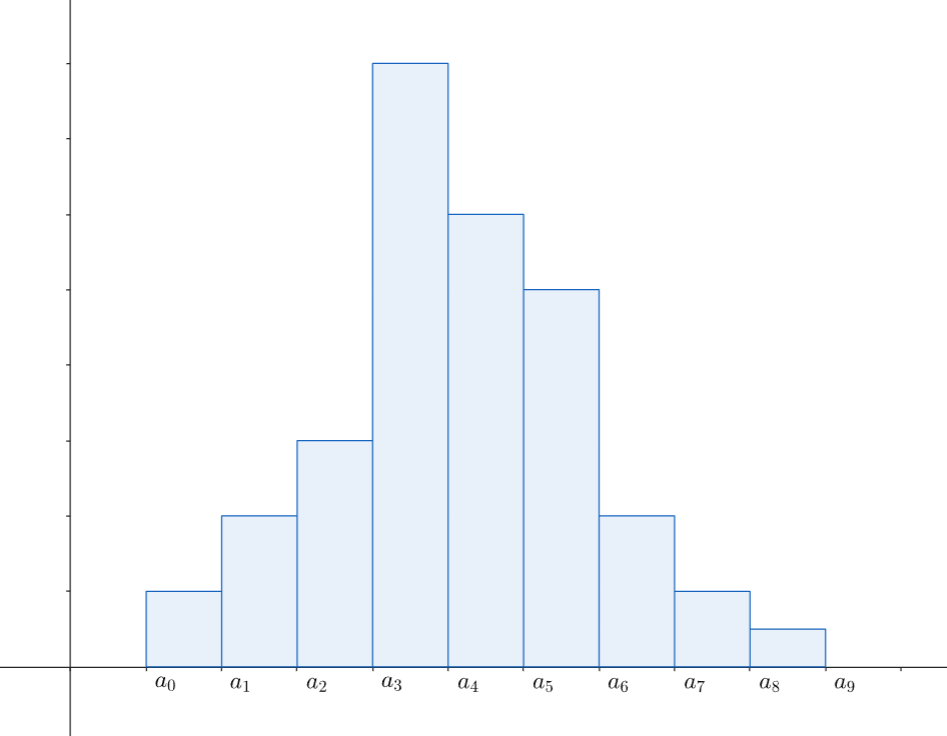
\includegraphics[width=0.4\textwidth]{mathstat/images/mathstat_2025_02_11_1}
            \end{center}

            \item Полигон

            На оси абсцисс отмечаем значения частотного вариационного ряда, по оси ординат - их частоты. 
            Получившиеся точки соединяем отрезками

            \begin{center}
                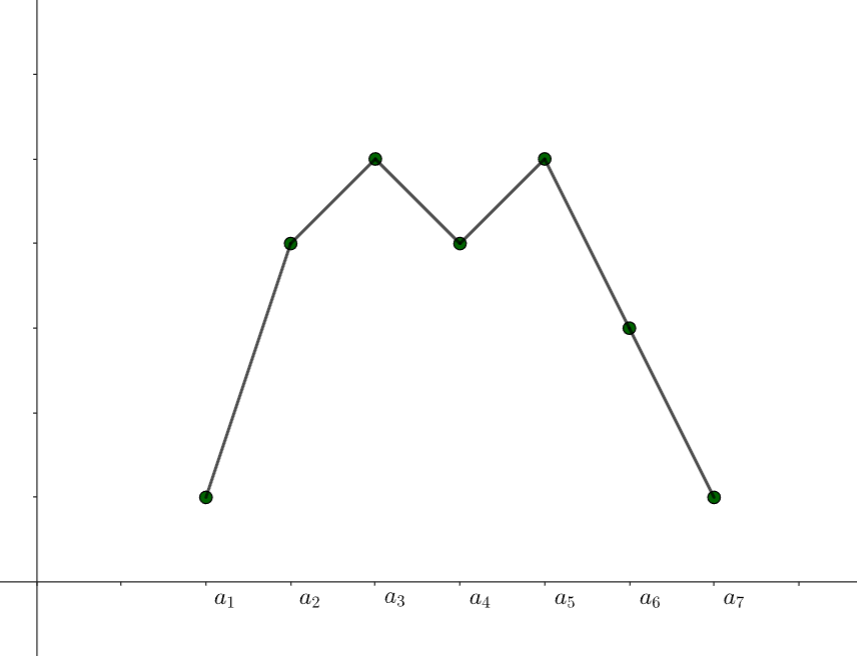
\includegraphics[width=0.4\textwidth]{mathstat/images/mathstat_2025_02_11_2}
            \end{center}
        \end{itemize}
    \end{multicols}

    \item Точечные оценки. Их свойства: состоятельность, несмещенность, эффективность.

    Пусть имеется выборка $\vec{X} = (X_1, X_2, \dots, X_n)$ объемом $n$. Пусть требуется найти приближенную оценку $\theta^*$ неизвестного параметра $\theta$. Находим ее при помощи некоторой функции обработки данных $\theta^* = \theta^*(X_1, \dots, X_n)$
    
    \Defs Такая функция называется статистикой
    
    \Defs А оценка $\theta^*$ называется \hyperlink{point_estimation}{точечной оценкой}

    \Defs Статистика $\theta^* = \theta^*(X_1, \dots, X_n)$ неизвестного параметра называется
    \textbf{состоятельной}, если $\theta^* \overset{p}{\longrightarrow} \theta$ при $n \to \infty$

    \Defs Оценка $\theta^*$ параметра $\theta$ называется \textbf{несмещенной}, если 
    математическое ожидание $E \theta^* = \theta$
        
    \Notas Оценка $\theta^*$ называется асимптотически несмещенной, если 
    $E \theta^* \overset{p}{\longrightarrow} \theta$ при $n \to \infty$

    \Defs Оценка $\theta^*_1$ не хуже $\theta^*_2$, если $E (\theta^*_1 - \theta)^2 \leq E (\theta^*_2 - \theta)^2$.
    Или, если $\theta^*_1$ и $\theta^*_2$ несмещенные, то $D \theta^*_1 \leq D \theta^*_2$

    \Defs Оценка $\theta^*$ называется \textbf{эффективной}, если она не хуже всех остальных оценок

    \Notas Не существует эффективной оценки в классе всех возможных оценок

    \begin{MyTheorem}
        \Ths В классе несмещенных оценок существует эффективная оценка
    \end{MyTheorem}

    \Defs Оценка $\theta^*$ параметра $\theta$ называется асимптотически нормальной, если 
    $\sqrt{n} (\theta^* - \theta) \rightrightarrows N(0, \sigma^2 (\theta))$ при $n \to \infty$

    \item Точечные оценки моментов. Свойства оценок математического ожидания и дисперсии.

    \hyperlink{moments_point_estimation}{Точечные оценки моментов}:

    \Defs Выборочным средним $\overline{x}$ называется величина $\overline{x} = \frac{1}{n} \sum_{i = 1}^n X_i$

    \Defs Выборочной дисперсией $D^*$ называется величина $D^* = \frac{1}{n} \sum_{i = 1}^n (X_i - \overline{x})^2$

    \Defs Исправленной дисперсией $S^2$ называется величина $S^2 = \frac{n}{n - 1} D^* = \frac{1}{n - 1} \sum_{i = 1}^n (X_i - \overline{x})^2$

    \Defs Выборочным средним квадратическим отклонением называется величина $\sigma^* = \sqrt{D^*}$

    \Defs Исправленным средним квадратическим отклонением называется величина $S = \sqrt{S^2}$

    \Defs Выборочным $k$-ым моментом называется величина $\overline{x^k} = \frac{1}{n} \sum_{i = 1}^n X_i^k$

    \Defs Модой $\mathrm{Mo}^*$ называется варианта $x_k$ с наибольшей частотой $n_k = \max_i (n_1, n_2, \dots, n_m)$

    \Defs Выборочной медианой $\mathrm{Me}^*$ называется варианта $x_i$ в середине вариационного ряда $\begin{cases}\mathrm{Me}^* = 
    X_{(k)}, & \text{если } n = 2k - 1 \\ \frac{X_{(k)} + X_{(k + 1)}}{2}, & \text{если } n = 2k\end{cases}$
    
    \begin{MyTheorem}
        \Ths $\overline{x}$ - состоятельная несмещенная оценка теоретического матожидания $EX = a$
    
        1) $E \overline{x} = a$
    
        2) $\overline{x} \overset{p}{\longrightarrow} a$ при $n \to \infty$
    \end{MyTheorem}
    
    \begin{MyTheorem}
        \Ths Выборочный $k$-ый момент является состоятельной несмещенной оценкой теоретического $k$-ого момента
    
        1) $\overline{E X^k} = E X^k$
    
        2) $\overline{X^k} \overset{p}{\longrightarrow} X^k$
    \end{MyTheorem}
    
    \begin{MyTheorem}
        \Ths Выборочной дисперсией $D^*$ и $S^2$ являются состоятельными оценками теоретической дисперсией, при этом $D^*$ - смещенная оценка, а $S^2$ - несмещенная оценка
    \end{MyTheorem}

    \item Метод моментов. Пример.

    \hyperlink{method_of_moments}{Метод моментов}: пусть имеется выборка объема $n$ неизвестного распределения, но известного типа,
    которое задается $k$ параметрами: $\theta = (\theta_1, \theta_2, \dots, \theta_k)$. Требуется дать оценки данным
    неизвестным параметрам

    Идея метода состоит в том, что сначала находим оценки $k$ моментов, а затем с помощью теоретических формул
    из теории вероятности даем оценки этих параметров

    Пусть $\vec{X}$ - выборка из абсолютно непрерывного распределения $F_\theta$ с плотностью известного типа, 
    которая задается $k$ параметрами $f_\theta (x, \theta_1, \dots, \theta_k)$

    Тогда теоретические моменты находим по формуле $m_i = \int_{-\infty}^{\infty} x^i f_\theta (x, \theta_1, \dots, \theta_k) dx = h_i(\theta_1, \dots, \theta_n)$

    Получаем систему из $k$ уравнений с $k$ неизвестными. В эти уравнения подставляем найденные оценки
    моментов и, решая получившуюся систему уравнений, находим нужные оценки параметров

    $\begin{cases}
    \overline{x} = h_1(\theta_1^*, \dots, \theta_n^*) \\ 
    \overline{x^2} = h_2(\theta_1^*, \dots, \theta_n^*) \\ 
    \dots \\
    \overline{x^k} = h_k(\theta_1^*, \dots, \theta_n^*) \\ 
    \end{cases}$

    \Ex Пусть $X \in U(a, b)$. Обработав статданные, нашли оценки первого и второго моментов: $\overline{x} = 2.25; \overline{x^2} = 6.75$

    Нужно найти оценки параметров $a^*, b^*$

    $EX = \int_a^b x \frac{1}{b - a} dx = \frac{a + b}{2}$

    $EX = \int_a^b x^2 \frac{1}{b - a} dx = \frac{a^2 + ab + b^2}{3}$

    Получаем:

    $\begin{cases}
        \overline{x} = \frac{a^* + b^*}{2} \\ 
        \overline{x^2} = \frac{a^*^2 + a^* b^* + b^*^2}{3} \\ 
    \end{cases} \Longleftrightarrow \begin{cases}
        a^* + b^* = 4.5 \\ 
        a^*^2 + a^* b^* + b^*^2 = 20.25 \\ 
    \end{cases} \Longleftrightarrow \begin{cases}
        a^* + b^* = 4.5 \\ 
        a^* b^* = 0 \\ 
    \end{cases} \Longleftrightarrow \begin{cases}
        a^* = 0 \\ 
        b^* = 4.5 \\ 
    \end{cases}$

    \item Метод максимального правдоподобия. Пример.

    \hyperlink{maximum_likelihood_estimation}{Метод максимального правдоподобия}: пусть имеется выборка $\vec{X} = (X_1, \dots, X_n)$ из распределения известного типа, определяемого неизвестными параметрами 
    $\theta = (\theta_1, \dots, \theta_n)$

    Идея метода состоит в следующем: подбираем параметры таким образом, чтобы вероятность получения
    данной выборки при случайном эксперименте была наибольшей.

    Если распределение дискретное, то $P_{\theta} (X_1 = x_1, X_2 = x_2, \dots, X_n = x_n) = P(X_1 = x_1) \dots P(X_n = x_n)$

    \Defs Функцией правдоподобия $L(\vec{X}, \theta)$ называется функция $L(\vec{X}, \theta) = P(X_1 = x_1) \dots P(X_n = x_n) = \prod_{i = 1}^n P(X_i = x_i)$ при дискретном распределении

    и $L(\vec{X}, \theta) = f_\theta(x_1) \dots f_\theta(x_n) = \prod_{i = 1}^n f_\theta(x_i)$ в абсолютно непрерывном распределении

    \Defs Логарифмической функцией правдоподобия называется функция $\ln L(\vec{X}, \theta)$

    \Notas Так как $y = \ln x$ возврастающая функция, точки максимума совпадают, а такую функцию правдоподобия становится легче дифференцировать

    \Defs Оценкой максимального правдоподобия $\hat{\theta}$ называется значение $\theta$, при котором функция правдоподобия 
    $L(\vec{X}, \theta)$ достигает наибольшего значения (при фиксированных значениях выборки)

    \Ex Пусть $\vec{X} = (X_1, \dots, X_n)$ - выборка из распределения Пуассона $\Pi_\lambda$ с неизвестным $\lambda > 0$

    \Mems Для распределения Пуассона $P(X = x_i) = \frac{\lambda^{x_i}}{x_i!} e^{-\lambda}$
    
    Получаем функцию максимального правдоподобия $L(\vec{X}, \lambda) = \prod_{i = 1}^n \frac{\lambda^{x_i}}{x_i!} e^{-\lambda} = 
    \frac{\lambda^{\sum_{i = 1}^n x_i}}{\prod_{i = 1}^n x_i!} e^{-n\lambda} = \frac{\lambda^{n \overline{x}}}{\prod_{i = 1}^n x_i!} e^{-n\lambda}$
    
    $\ln L(\vec{X}, \lambda) = n \overline{x} \ln \lambda - \ln \prod_{i = 1}^n x_i! - n\lambda$
    
    $\frac{\partial \ln L}{\partial \lambda} = \frac{n \overline{x}}{\lambda} - n = 0 \Longrightarrow \hat{\lambda} = \overline{x}$ - оценка максимального правдоподобия
    
    Убедимся, что этот экстремум - максимум: $\frac{\partial^2 \ln L}{\partial \lambda^2} = -\frac{n \overline{x}}{\lambda} < 0 \Longrightarrow \hat{\lambda} = \overline{x}$ - точка максимума
    
    \item Информация Фишера. Неравенство Рао-Крамера (без док-ва).

    Пусть $X \in F_\theta$ - семейство распределений с параметром $\theta \in \Real$

    \Def Носителем семейства распределений $F_\theta$ называется множество $C \subset \Real$
    такое, что $P(X \in C) = 1 \ \forall X \in F_\theta$

    $f_\theta(x) = \begin{cases}
        \text{плотность } f_\theta(x) \text{ при непрерывном распределении} \\
        P_\theta(X = x) \text{ при дискретном распределении}
    \end{cases}$

    \Def \hyperlink{fishers_information}{Информацией Фишера} $I(\theta)$ семейства распределений $F_\theta$ называется величина 
    $I(\theta) = E\left(\frac{\partial}{\partial \theta} \ln f_\theta(X)\right)^2$ при условии, что
    она существует

    \Def Семейство распределений $F_\theta$ называется регулярным, если:

    \begin{itemize}
        \item существует носитель $C$ семейства $F_\theta$ такой, что $\forall x \in C \ $ функция $\ln f_\theta(x)$ непрерывно дифференцируема по $\theta$
        \item информация Фишера $I(\theta)$ существует и непрерывна по $\theta$
    \end{itemize}

    \begin{MyTheorem}
        \ThNs{\hyperlink{rao_kramer_inequality}{Неравенство Рао-Крамера}} Пусть $(X_1, \dots, X_n)$ - выборка объема $n$ из регулярного семейства $F_\theta$,

        $\theta^* = \theta^*(X_1, \dots, X_n)$ - несмещенная оценка параметра $\theta$, дисперсия которой
        $D\theta^*$ ограничена в любой замкнутой ограниченной области параметра $\theta$

        Тогда \fbox{$D\theta^* \geq \frac{1}{n I(\theta)}$}
    \end{MyTheorem}

    \underline{Следствие}: если при данных услових получили $D\theta^* = \frac{1}{n I(\theta)}$, то оценка $\theta^*$ является эффективной 
    (то есть дальше улучшать уже некуда)

    \item Основные распределения математической статистики: хи-квадрат, Стьюдента, Фишера-Снедекора. Их свойства.

    \Def Распределение \enquote{хи-квадрат} $H_n$ со степенями свободы $n$ называется распределение
    суммы квадратов независимых стандартных нормальных величин: $\chi^2_n = X_1^2 + X_2^2 + \dots + X_n^2$, 
    где $X \in N(0, 1)$ и независимы

    \underline{Свойства}

    \begin{enumerate}
        \item $E\chi^2_n = n$

        \begin{MyProof}
            Так как $\forall i \ X_i \in N(0, 1)$, то $E X_i^2 = D X_i^2 + (EX_i)^2 = 1 \Longrightarrow E(X_i^2 + \dots X_n^2) = \sum_{i = 1}^n E X_i^2 = n$
        \end{MyProof}

        \item Устойчивость относительно суммирования: если $X \in H_n$, $Y \in H_m$, независимы, то $X + Y \in H_{n + m}$ (по определению) 


        \item $\frac{\chi_k^2}{k} \overset{p}{\underset{k \to \infty}{\longrightarrow}} 1$ (по Закону Больших Чисел)
    \end{enumerate}

    \Def Пусть $X_0, X_1, \dots, X_k$ - независимые стандартные нормальные величины. 
    Распределением Стьюдента $T_k$ с $k$ степенями свободы называется распределение случайной величины 
    $t_k = \frac{X_0}{\sqrt{\frac{1}{k} (X_1^2 + \dots + X_k^2)}} = \frac{X_0}{\sqrt{\frac{\chi_k^2}{k}}}$

    \underline{Свойства}

    \begin{enumerate}
        \item $Et_k = 0$ - в силу симметрии

        \item $t_k \rightrightarrows N(0, 1)$ (на практике при $k \geq 100$ распределение Стьюдента можно считать стандартным нормальным)
    \end{enumerate}

    \Def Распределением Фишера-Снедекера $F_{n,m}$ (другое название - F-распределение) со степенями свободы $n$ и $m$ называется распределение случайной величины 
    $f_{n,m} = \frac{\frac{\chi^2_n}{n}}{\frac{\chi^2_m}{m}}$, где $\chi_n^2$ и $\chi_m^2$ - независимые случайные величины с распределением \enquote{хи-квадрат}

    \underline{Свойства}

    \begin{enumerate}
        \item $E f_{n,m} = \frac{n}{n - 2}$

        \item $f_{n,m} \overset{p}{\underset{n, m \to \infty}{\longrightarrow}} 1$
    \end{enumerate}

    \item Линейные преобразования нормальных выборок. Теорема об ортогональном преобразовании.

    \Def Пусть случайный вектор $\vec \xi = \begin{pmatrix}\xi_1 \\ \vdots \\ \xi_n\end{pmatrix}$ имеет вектор средних 
    $\vec a = E \vec \xi$, $K$ - симметричная положительно определенная матрица. Вектор $\vec \xi$ 
    имеет нормальное распределение в $\Real^n$ с параметрами $\vec a$ и $K$, если его плотность 
    $f_{\vec \xi} (\vec X) = \frac{1}{\left(\sqrt{2\pi}\right)^n \sqrt{\det K}} e^{-\frac{1}{2} (\vec X - \vec a)^T K^{-1} (\vec X - \vec a)}$


    \underline{Свойства}

    \begin{enumerate}
        \item Матрица $K = D \vec \xi = \left(\mathrm{cov} (\xi_i, \xi_j)\right)$ - матрица ковариаций

        \item При $\vec a = \vec 0$ и $K = E$ имеем вектор из независимых стандартных нормальных величин

        \begin{MyProof}
            При $\vec a = \vec 0$ и $K = E$: $f_{\vec \xi} (X_1, \dots, X_n) = \frac{1}{\left(\sqrt{2\pi}\right)^n} 
            e^{-\frac{1}{2} \begin{pmatrix}X_1 & \dots & X_n\end{pmatrix} E \begin{pmatrix}X_1 & \dots & X_n\end{pmatrix}^T} = 
            \frac{1}{\left(\sqrt{2\pi}\right)^n} e^{-\frac{1}{2} (X_1^2 + \dots + X_n^2)} = 
            \frac{1}{\sqrt{2\pi}} e^{-\frac{1}{2} X_1^2} + \dots + \frac{1}{\sqrt{2\pi}} e^{-\frac{1}{2} X_n^2}$

            Так как плотность распалась на произведение плотностей стандартного нормального распределение, то все компоненты имеют стандартное нормальное распределение
        \end{MyProof}

        \item $\letsymbol \vec X$ - стандартный нормальный вектор, $B$ - невырожденная матрица, 
        тогда вектор $\vec Y = B \vec X + \vec a$ имеет многомерное нормальное распределение с параметрами $\vec a$ и $K = B B^T$

        \item $\letsymbol \vec Y \in N(\vec a, K)$. Тогда вектор $\vec X = B^{-1} (\vec Y - \vec a)$ - стандартный нормальный вектор, где $B = \sqrt{K}$

        \underline{Следствие}. Эквивалентное определение: Многомерное нормальное распределение - это то, которое получается из
        стандартного нормального вектора при помощи невырожденного преобразования и сдвига

        \item $\letsymbol \vec X$ - стандартный нормальный вектор, $C$ - ортогональная матрица. Тогда $\vec Y = C \vec X$ - стандартный нормальный вектор

        \begin{MyProof}
            Так как $C$ - ортогональная, то $C^T = C^{-1}$. Тогда по третьему свойству $K = C C^T = E$, а по второму свойству $\vec Y$ - стандартный нормальный вектор
        \end{MyProof}

        \item $\letsymbol$ случайный вектор $\xi \in N(\vec a, K)$.
        Тогда его координаты независимы тогда и только тогда, когда они не коррелированы (то есть матрица ковариаций $K$ диагональная)

        % какого распределения величины
        \underline{Следствие}. Если плотность совместного распределения случайных величин $\xi$ и $\eta$ ненулевая, то они независимы тогда и только тогда, 
        когда их коэффициент корреляции равен нулю
    \end{enumerate}

    \item Лемма Фишера.

    \begin{MyTheorem}
        \Ths{\hyperlink{fishers_lemma}{Лемма Фишера}} Пусть вектор $\vec X$ - стандартный нормальный вектор, $C$ - ортогональная матрица, $\vec Y = C \vec X$.
        Тогда $\forall 1 \leq k \leq n - 1 \ $ случайная величина $T(\vec X) = \sum_{i = 1}^n X_i^2 - Y_1^2 - Y_2^2 - \dots Y_k^2$ 
        не зависит от $Y_1, Y_2, \dots, Y_k$ и имеет распределение \enquote{хи-квадрат} со степенями свободы $n - k$
    \end{MyTheorem}

    \begin{MyProof}
        Так как $C$ - ортогональное преобразование, то $\|\vec X\| = \|\vec Y\|$, то есть $\sum_{i = 1}^n X^2_i = \sum_{i = 1}^n Y^2_i \Longrightarrow
        T(\vec X) = \sum_{i = 1}^n X_i^2 - Y_1^2 - Y_2^2 - \dots Y_k^2 = Y^2_{k + 1} + \dots + Y^2_{n}$

        Согласно свойству 5 $Y_i \in N(0, 1)$ и независимы, то по определению \enquote{хи-квадрат} $T(\vec X) \in H_{n - k}$ и не зависит от $Y_1, \dots, Y_k$
    \end{MyProof}

    \item Основная теорема о связи точечных оценок нормального распределения и основных распределений статистики.

    \begin{MyTheorem}
        \Ths Пусть $(X_1, \dots, X_n)$ - выборка из нормального распределения $N(a, \sigma^2)$, $\overline{x}$ - выборочное среднее, $S^2$ - исправленная дисперсия.

        Тогда справедливы следующие высказывания:

        \begin{enumerate}
            \item $\sqrt{n} \frac{\overline{x} - a}{\sigma} \in N(0, 1)$
            
            \item $\sum_{i = 1}^n \frac{(X_i - a)^2}{\sigma^2} \in H_n$
            
            \item $\sum_{i = 1}^n \frac{(X_i - \overline{x})^2}{\sigma^2} = \frac{n D^*}{\sigma^2} = \frac{(n - 1) S^2}{\sigma^2} \in H_{n - 1}$

            \item $\sqrt{n} \frac{\overline{x} - a}{S} \in T_{n - 1}$
            
            \item $\overline{x}$ и $S^2$ независимы
        \end{enumerate}
    \end{MyTheorem}

    \item Квантили распределений (оба определения). Функции для их вычисления в EXEL.
    \item Интервальные оценки. Определения, смысл, терминология.
    \item Доверительный интервал для математического ожидания нормального распределения при известном $\sigma$.
    \item Доверительный интервал для математического ожидания нормального распределения при неизвестном $\sigma$.
    \item Доверительный интервал для дисперсии нормального распределения при неизвестном $a$.
    \item Доверительный интервал для дисперсии нормального распределения при известном $a$.
    \item Проверка статистических гипотез. Определения, терминология. Уровень значимости и мощность критерия.
    \item Способы сравнения критериев проверки гипотез.
    \item Построение критериев согласия (основные принципы).
    \item Гипотеза о среднем нормальной совокупности с известной дисперсией.
    \item Гипотеза о среднем нормальной совокупности с неизвестной дисперсией.
    \item Доверительные интервалы как критерии гипотез о параметрах распределения.
    \item Критерий хи-квадрат для параметрической гипотезы.
    \item Критерий хи-квадрат для гипотезы о распределении.
    \item Критерий Колмогорова для гипотезы о распределении.
    \item Критерий Колмогорова-Смирнова.
    \item Критерий Фишера.
    \item Критерий Стьюдента.
    \item Понятие статистической зависимости. Корреляционное облако и корреляционная таблица. Первоначальные выводы.
    \item Критерий хи-квадрат для проверки независимости.
    \item Однофакторный дисперсионный анализ. Общая, межгрупповая и внутригрупповая дисперсии. Теорема о разложении дисперсии.
    \item Однофакторный дисперсионный анализ. Проверка гипотезы о влиянии фактора.
    \item Математическая модель регрессии. Основные понятия и определения. Метод наименьших квадратов.
    \item Вывод уравнения линейной парной регрессии. Геометрический смысл прямой регрессии.
    \item Выборочный коэффициент линейной корреляции. Проверка гипотезы о его значимости.
    \item Выборочное корреляционное отношение, его свойства.
    \item Свойства ошибок в модели линейной парной регрессии. Анализ дисперсии фактора-результата. Коэффициент детерминации, его свойства.
    \item Проверка гипотезы о значимости уравнения линейной регрессии. Связь между коэффициентом детерминации и коэффициентом линейной корреляции.
    \item Теорема Гаусса-Маркова.
    \item Стандартные ошибки коэффициентов регрессии. Их доверительные интервалы.
    \item Прогнозирование в модели линейной парной регрессии. Стандартная ошибка прогноза, доверительный интервал прогноза.
    \item Общая модель линейной регрессии. Вывод нормального уравнения.
    \item Свойства ОНМК в уравнении общей линейной регрессии.
    \item Основная теорема об ОМНК (п.2 без доказательства).
    \item Мультиколлинеарность, ее неприятные последствия. Основные принципы отбора факторов в модель общей линейной регрессии.
    \item Стандартная ошибка общей линейной регрессии и стандартные ошибки коэффициентов регрессии. Проверка гипотезы о значимости отдельного коэффициента регрессии.
    \item Уравнение регрессии в стандартных масштабах. Смысл стандартизованных коэффициентов. Разложение влияния фактора на прямое и косвенное.
    \item Коэффициенты детерминации и множественной корреляции, их свойства. Проверка гипотезы о значимости уравнения регрессии в целом.
    \item Взвешенный МНК.
    \item Приемы сведения нелинейных регрессий к линейным.
    \item Математические датчики случайных чисел.
    \item Моделирование случайных величин методом обратной функции (включая дискретный случай).
    \item Моделирование нормальной случайной величины.
    \item Быстрый показательный датчик.
    \item Моделирование дискретных случайных величин.
    \item Метод Монте-Карло. Общая постановка, оценка погрешности.
    \item Вычисление определенного и кратного интегралов методом Монте-Карло. Метод расслоенной выборки.
\end{enumerate}
